\chapter{Đại số cơ bản}

\section{Ánh xạ}

Cho 2 tập hợp $X$ và $Y$. Ánh xạ $f$ biến một phần tử $x \in X$ thành một và chỉ một phần tử $y \in Y$.

Ta ký hiệu
\[f: X \rightarrow Y, \; f(x) = y\]

Khi đó, $X$ được gọi là tập nguồn (domain) và $Y$ là tập đích (image).

Ánh xạ có 3 loại:

\begin{itemize}[noitemsep]
    \item Đơn ánh (Injection): Hai phần tử khác nhau của tập nguồn cho hai ảnh khác nhau. Tức là với mọi $x_1, x_2 \in X$ mà $x_1 \neq x_2$, thì $f(x_1) \neq f(x_2)$
    \item Toàn ánh (Surjection): Mọi phần tử $y \in Y$ đều có ít nhất một phần tử $x \in X$ mà $f(x) = y$. Nói cách khác với mỗi phần tử trong $Y$ ta đều tìm được phần tử thuộc $X$ biến thành nó
    \item Song ánh (Injection): Nếu ánh xạ đó vừa là đơn ánh, vừa là toàn ánh
\end{itemize}

\begin{remark}
    Dựa vào định nghĩa và hình vẽ, ta có thể rút ra kết luận như sau
    \begin{itemize}[noitemsep]
        \item Đối với đơn ánh, do mọi phần tử của $X$ đều có ảnh ở $Y$, tuy nhiên có thể có phần tử ở $Y$ không do phần tử nào của $X$ biến thành (trong hình là 5). Do đó $| X | \leq | Y |$
        \item Đối với toàn ánh, mọi phần tử của $Y$ đều có nguồn gốc xuất xứ, tuy nhiên có thể có phần tử của $X$ không biến thành $y$ nào của $Y$ (trong hình là $e$). Do đó $| X | \geq | Y |$
        \item Đối với song ánh, do là kết hợp giữa đơn ánh và toàn ánh, khi đó dấu đẳng thức xảy ra, $| X | = | Y |$
    \end{itemize}
\end{remark}

\begin{figure}[ht]
    \centering
    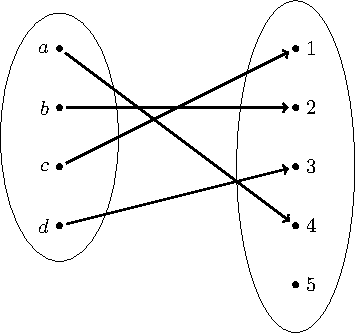
\includegraphics{pics/maps/injection.pdf}
    \caption{Đơn ánh}
\end{figure}

\begin{figure}[ht]
    \centering
    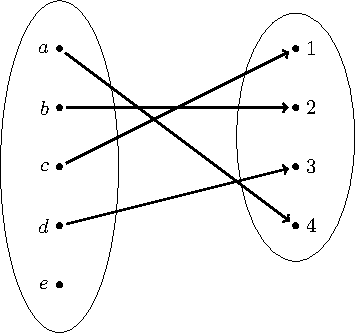
\includegraphics{pics/maps/surjection.pdf}
    \caption{Toàn ánh}
\end{figure}

\begin{figure}[ht]
    \centering
    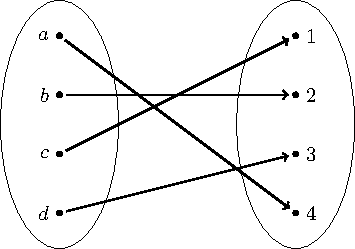
\includegraphics{pics/maps/bijection.pdf}
    \caption{Song ánh}
\end{figure}

\section{Hàm số}

Khi 2 tập nguồn và đích của ánh xạ là 2 tập hợp số, ta có hàm số.

\begin{example}
    Hàm số $f: \RR \rightarrow \RR$ với $y = f(x) = x^3 + x + 1$. Ở đây $X \equiv \RR$ và $Y \equiv \RR$.
\end{example}

Lưu ý rằng tập nguồn và đích không nhất thiết là tập hợp số cơ bản ($\QQ, \RR$) mà cũng có thể là tích Descartes của chúng.

\begin{example}
    Hàm số $f: \RR \times \RR \rightarrow \RR$ với $z = f(x, y) = x + y + xy$. Ở đây $X \equiv \RR$, $Y \equiv \RR$ và $Z \equiv \RR$.
\end{example}

Chúng ta còn một cách gọi khác cho đơn ánh, toàn ánh, song ánh trong tiếng Anh.

\begin{table}[ht]
    \centering
    \begin{tabular}{| l | l | l |}
        \hline
        đơn ánh & injection & one-to-one map \\
        \hline
        toàn ánh & surjection & onto map \\
        \hline
        song ánh & bijection & one-to-one and onto map \\
        \hline
    \end{tabular}

    \caption{Thuật ngữ tiếng Anh cho ánh xạ}
\end{table}

\begin{example}
    Hàm số $f: \RR \rightarrow \RR$ cho bởi $y = f(x) = x^3$ là song ánh.

    \begin{proof}
        Ta thấy nếu $f(x_1) = f(x_2)$, tương đương $x_1^3 = x_2^3$ nên $x_1 = x_2$. Do đó $f$ là đơn ánh.

        Với mọi $y = x^3 \in \RR$, do căn bậc 3 luôn tồn tại nên ta có $x = \sqrt{3}{y}$. Nghĩa là luôn tồn tại $x$ để $f(x) = y$ với mọi $y \in \RR$. Do đó $f$ là toàn ánh.

        Kết luận $f$ là song ánh.
    \end{proof}
\end{example}

